\documentclass{article}
\usepackage{graphicx} % Required for inserting images
\usepackage[utf8]{inputenc}
\usepackage{amsmath,amsfonts,amssymb,amsthm}
\usepackage{enumerate,bbm}
\usepackage{leftindex}
\usepackage{tikz,tikz-cd,graphicx,color,mathrsfs,color,hyperref,boldline}
\usepackage{caption,float}
\usepackage[a4paper,margin=1in,footskip=0.25in]{geometry}

\usepackage{listings}
\usepackage{xcolor}

\usepackage{tabularx,capt-of}

\usepackage{blindtext}
%Image-related packages
\usepackage{graphicx}
\usepackage{subcaption}
\usepackage[export]{adjustbox}
\usepackage{lipsum}

%hyperref setup
\hypersetup{
    colorlinks=true,
    linkcolor=blue,
    filecolor=magenta,      
    urlcolor=cyan,
    pdftitle={Overleaf Example},
    pdfpagemode=FullScreen,
    }

%New colors defined below
\definecolor{codegreen}{rgb}{0,0.6,0}
\definecolor{codegray}{rgb}{0.5,0.5,0.5}
\definecolor{codepurple}{rgb}{0.58,0,0.82}
\definecolor{backcolour}{rgb}{0.95,0.95,0.92}

%Code listing style named "mystyle"
\lstdefinestyle{mystyle}{
  backgroundcolor=\color{backcolour}, commentstyle=\color{codegreen},
  keywordstyle=\color{magenta},
  numberstyle=\tiny\color{codegray},
  stringstyle=\color{codepurple},
  basicstyle=\ttfamily\footnotesize,
  breakatwhitespace=false,         
  breaklines=true,                 
  captionpos=b,                    
  keepspaces=true,                 
  numbers=left,                    
  numbersep=5pt,                  
  showspaces=false,                
  showstringspaces=false,
  showtabs=false,                  
  tabsize=2
}

%"mystyle" code listing set
\lstset{style=mystyle}

\theoremstyle{definition}
\newtheorem{defn}{Definition}[section]
\newtheorem{example}[defn]{Example}
\theoremstyle{remark}
\newtheorem{rem}{Remark}
\newtheorem{remS}[section]{defn}
\theoremstyle{plain}
\newtheorem{lem}[defn]{Lemma}
\newtheorem{thm}[defn]{Theorem}
\newtheorem{prop}[defn]{Proposition}
\newtheorem{fact}[defn]{Fact}
\newtheorem{crly}[defn]{Corollary}
\newtheorem{conj}[defn]{Conjecture}

%\newtheorem*{programming*}{Programming Task}

%\newtheorem{innercustomgeneric}{\customgenericname}
%\providecommand{\customgenericname}{}
%\newcommand{\newcustomtheorem}[2]{%
%  \newenvironment{#1}[1]
%  {%
%   \renewcommand\customgenericname{#2}%
%   \renewcommand\theinnercustomgeneric{##1}%
%   \innercustomgeneric
%  }
%  {\endinnercustomgeneric}
%}

%\newcustomtheorem{question}{Question}
%\newcustomtheorem{programming}{Programming Task}

\newcommand{\NN}{\mathbb{N}}
\newcommand{\ZZ}{\mathbb{Z}}
\newcommand{\QQ}{\mathbb{Q}}
\newcommand{\RR}{\mathbb{R}}
\newcommand{\CC}{\mathbb{C}}
\newcommand{\PP}{\mathbb{P}}
\newcommand{\FF}{\mathbb{F}}
\newcommand{\Hom}{\operatorname{Hom}}
\newcommand{\im}{\operatorname{im}}
\newcommand{\id}{\operatorname{id}}
\newcommand{\Ind}{\operatorname{Ind}}
\newcommand{\Res}{\operatorname{Res}}
\newcommand{\btop}{\mathbf{Top}}
\newcommand{\bdel}{\mathbf{\Delta}}
\newcommand{\sing}{\operatorname{Sing}}
\newcommand{\bset}{\mathbf{Set}}
\newcommand{\Rmod}{\mathbf{Mod}_R}
\newcommand{\colim}{\operatorname{colim}}

\newcommand{\calD}{\mathcal{D}}

\newcommand{\sol}{\textit{Solution: }}

\title{Simplicial Homotopy Theory}
\author{Kevin}
\date{January 2025}

\begin{document}
\maketitle
\section{Introduction}
Recall basic notions from category theory
\begin{defn}
    A category $\mathscr{C}$ consists of a collection of objects, denoted $\operatorname{ob}(\mathscr C)$, and for each pair of objects $A,B$, a collection of morphisms $\Hom_{\mathscr C}(A,B)$ such that
    \begin{itemize}
        \item [(i)] There is an associative composition law of morphisms.
        \item[(ii)] For each $A\in\operatorname{ob}(\mathscr C)$, there is a distinguished element $\id_A\in\Hom_{\mathscr C}(A,A)$, which is left and right unital.
    \end{itemize}
\end{defn}
\begin{defn}
    A morphism is called an isomorphism if it has a two-sided inverse.
\end{defn}

Given a category $\mathscr{C}$, want to classify objects up to isomorphism.

For the purpose of this course, $\mathbf{Top}$ will denote the category  with objects those topological spaces that are homeomorphic to a CW complex. Morphisms are cts functions. Isomorphisms are homeomorphisms. We might attempt to classify objects in $\mathbf{Top}$ up to homeo.

A useful tool is a functor, for every integer $i$ and commutative irng $R$
\[H_i(-;R):\mathbf{Top}\to\Rmod,\ X\mapsto H_i(X;R)\]
A key ingredient in the defns of these functors is the study of cts maps from the n-simplex into $X$, as $n$ varies.

There is a factorization of functors.
\[H_i(-;R):\mathbf{Top}\to \mathbf{HoTop}\to\Rmod\]
where $\mathbf{HoTop}$ is the full subcategory of $\mathbf{Top}$ obtained by forcing homotopic cts maps to be equal (so an isomoprhism in this category is a htpy equivalence). Homotopy theory is the study of $\mathbf{HoTop}$.
\begin{rem}
    Isomorphism classes in $\mathbf{HoTop}$ can be understood via the moduli stack of formal groups and other objects in arithmetic geometry.
\end{rem}

\textbf{Question: How to think about objects in $\mathbf{HoTop}$ up to isomorphism?}

Roughly, a homotopy type consists of 
\begin{itemize}
    \item A collection of objects
    \item For every pair of objects a collection of isomorphism between them
    \item For every pair of parallel isomorphism $f,g:A\to B$ a collection of 2-isomorphisms between them.
\end{itemize}
\begin{example}
    The following shows two different homotopy types.
    \begin{figure}[H]
        \centering
        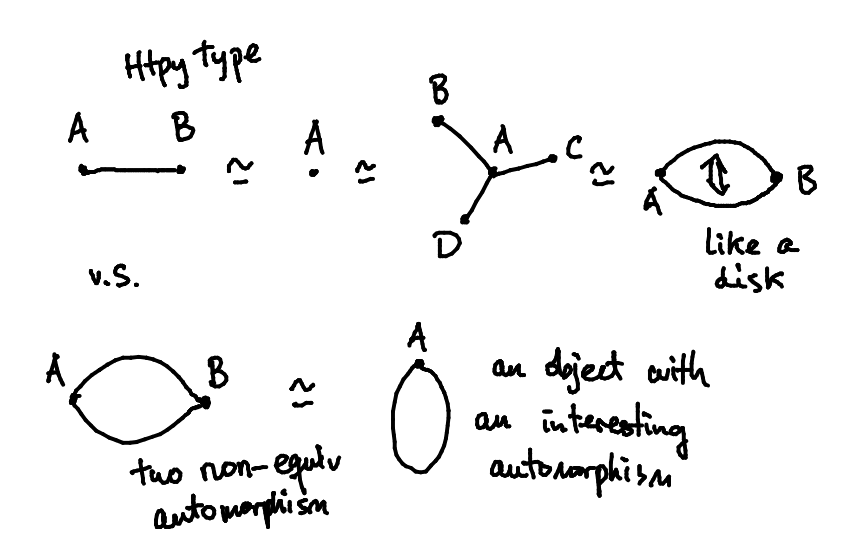
\includegraphics[width=0.5\linewidth]{Lent/pictures/htpy_type_example.PNG}
        \caption{Two different homotopy types}
        \label{fig:1}
    \end{figure}
    On the top, we have a homotopy type consisting of two objects $A, B$ and an isomorphism between them (represented by the edge). This is isomorphic to a single object $A$ as we can (formally) contract the isomorphism to identify equivalent objects. It is also equivalent to a htpy type consisting of $A,B,C,D$ where $B,C,D$ are all isomorphic to $A$ via a unique isomorphism. It is also euqivalent to the htpy type consisting of two objects $A,B$, two isomorphisms $A\to B$ and a 2-isomorphism, i.e., an equivalence of these two isomorphisms.

    On the bottom, we have another homotopy type with two objects and two non-equivalent isomorphisms. We may contract one isomoprhism and get a htpy type of consisting of a single object with an interesting automorphism.

    Sets are homotopy types with no non-trivial isomoprhisms or 2-isomorphisms.

    Groupoids, i.e., categories in which all morphisms are isomorphisms, are homotopy types with no non-trivial 2-isomorphisms and 3-isomorphisms, etc.
\end{example}
Given a topological space $X$, there is an associated homotopy type s.t.
    \begin{itemize}
        \item points of $X$ are objects. (cts maps from the $0$-simplex)
        \item paths in $X$ are isomorphisms. (cts maps from the $1$-simplex)
        \item A cts function $|\Delta^2|\to X$ is a 2-isomorphism. (Regard the map restricted to two edges of $|\Delta^2|$ as a concatenation of paths, then the map is essentially a homotopy rel the boundary of $|\Delta^1|$.)
    \end{itemize}

We want to study homotopy types. These can be presented as topological spaces (that are homeo to CW complexes) up to homotopy equivalence. SInce spaces are complicated unwieldy objects, we will seek to describe homotopy types in combinatorial terms. We will desribe homotopy types as special sorts of simplicial sets up to an appropriate notion of equivalence.

\begin{defn}
    The simplex category $\mathbf{\Delta}$ has 
    \begin{itemize}
        \item objects $[n]$ for every integer $n\ge 0$
        \item A morphism $[n]\to[m]$ is an order preserving function from $\{1\le2\le...\le n\}\to\{1\le 2\le...\le m\}$.
    \end{itemize}
\end{defn}
There is a functor $\mathbf{\Delta}\to\mathbf{Top}$ sending $[n]\mapsto|\Delta^n|$. This is a good way to visualize $\bdel$. We introduce some special notations for certain morphisms in $\bdel$.
\begin{itemize}
    \item Face maps: $\delta^i:[n-1]\to[n]$ is the order preserving injection that omits $i$.
    \item Degeneracy maps: $\sigma^i:[n+1]\to[n]$ is the order preserving surjection that hits $i$ twice.
\end{itemize}
\begin{rem}
    Every morphism in $\bdel$ is a composite of face and degeneracy maps.
\end{rem}

\begin{defn}
    A simplicial set is a functor $\mathbf{\Delta}^{op}\to\mathbf{Set}$. A morphism of simplicial sets is a natural transformation. There is a category of simplicial sets, denoted $s\bset$.
\end{defn}
Explicitly, a simplicial set $X:\bdel^{op}\to \bset$ is a collection of sets $X_0,X_1,X_2,...$, where $X_i=X([i])$ with maps of sets $d_0,...,d_n:X_n\to X_{n-1}$ and $s_0,...,s_n:X_{n}\to X_{n+1}$ satisfying the following simplicial identities:
\begin{align*}
    &d_id_j=d_{j-1}d_i,\ \ i<j\\
    &d_is_j=s_jd_{i-1},\ \ i<j\\
    &d_is_j=s_{j}d_{i+1},\ \ i>j+1\\
    &s_is_j=s_{j+1}s_i,\ \ i<j
\end{align*}
\begin{example}
    If $X$ is a topological space, there is an associated simplicial set $\sing(X):\mathbf{\Delta}^{op}\to \mathbf{Set}$ which sends $[n]$ to the set of continuous functions $|\Delta^n|\to X$. So $\sing(X)_n=\Hom_{\btop}(|\Delta^n|,X)$.
\end{example}
\begin{rem}
    Not every simplicial set is $\sing$ of some topological space. $C_\ast^{\sing}(X;R)$ depends only on $\sing(X)$.
\end{rem}

\begin{defn}
    For every integer $n\ge 0$, there is a simplicial set denoted $\Delta^n$ defined as $(\Delta^n)_m=\Hom_\bdel([n],[m])$.
\end{defn}
Yoneda lemma implies that $\Hom_{s\bset}(\Delta^n,X)\cong X_n$ as sets for any simplicial set $X$.
\begin{rem}
    If $\mathscr{C}$ is any (small) category, the category of presheaves on $\mathscr C$ is the category of functors $\mathscr C^{op}\to\bset$. The Yoneda embedding is a functor $y:\mathscr C\to\operatorname{Psh}(\mathscr C),\ c\mapsto (c'\mapsto \Hom_{\mathscr C}(c',c))$.

    In this particular situation, $s\bset=\operatorname{Psh}(\bdel)$ and $\Delta^n=y([n])$.
\end{rem}
\begin{rem}
    Another feature of presheaf categories is that any $X\in\operatorname{Ob}(\operatorname{Psh}(\mathscr C))$ can be written as a colimit of objects in the image of the Yoneda embedding. We will appl this to $s\bset$.
\end{rem}
Let $I$ denotes the category with objects maps $\Delta^n\to X$ for any $n$ and morphisms commuting diagrams:
\begin{center}
    % https://tikzcd.yichuanshen.de/#N4Igdg9gJgpgziAXAbVABwnAlgFyxMJZABgBpiBdUkANwEMAbAVxiRAB12ARGBnOgHqEAvqXSZc+QigCM5KrUYs2ADQD6nAEZMGDGDhCjx2PASJkZC+s1aIO3XvwEBbQwphQA5vCKgAZgBOEK6IZCA4EEgATNTWyohgOgzUDHSavAAKEqbSIHp+BkYggcFIYRFIcoo2SIm6KWmZ2VJs+YVixUEhMeGRiFVxtnXJeY0MWSYtdm1uwkA
\begin{tikzcd}
\Delta^n \arrow[d] \arrow[r] & X_\bullet \\
\Delta^m \arrow[ru]          &          
\end{tikzcd}
\end{center}

Now consider the functor $I\to\bdel$, $(\Delta^n\to X_\bullet)\mapsto [n]$. Compose this with the Yoneda functor $y:\bdel\to s\bset$. We then get a functor $F:I\to s\bset$. Then $X_\bullet=\operatorname{colim}(F)$.


\begin{defn}
    Geometric realization is a functor $|\cdot |:s\bset\to\btop$.
\end{defn}
\begin{rem}
    It is the unique colimit preserving functor taking $\Delta^n$ to $|\Delta^n|$. (The previous discussion shows that if such functor exists then it's unique) We will construct this functor later :).
\end{rem}
This functor will allow us to visualize simplicial sets constructed by combinatorial means.
\begin{rem}
    If $X$ is a nice top. space, then $\sing(X)$ is a combinatorial model for the htpy type of $X$.
    Similarly, if $Y$ is a ``nice'' simplicial set, then $|Y|$ is a top. model for the htpy type of $Y$. In particular, if $X$ is a nice space then $|\sing(X)|$ is htpy equivalent to $X$.
\end{rem}
\begin{example}
    For every $n\ge0$, $\partial\Delta^n$ is a simplicial set with $(\partial \Delta^n)_m=\Hom_{s\bset}(\Delta^n,\partial\Delta^n)=\{\alpha:[m]\to[n]:\text{not surjective}\}$. There is a canonical map $\partial\Delta^n\to\Delta^n$
\end{example}
\begin{prop}
    The geometric realization $|\partial\Delta^n\to\Delta^n|$ is the inclusion of the boundary of the standard $n$-simplex.
\end{prop}
\begin{proof}
    If $n=1$, then any non-surjective order preserving function is constantly $0$ or $1$.

    If $n\ge 2$, then we have
    \[\partial \Delta^n=\operatorname{colim}\left(\coprod_{0\le i<j\le n}\Delta^{n-2}\overset{\rightarrow}{\rightarrow}\coprod_{0\le i\le n}\Delta^{n-1}\right)\]
\end{proof}
\begin{example}
    For $n\ge1$ and $-\le i\le n$, we define $\Lambda_i^n$, the $i$th horn in $\Delta^n$ to send $[m]$ to the set of order-preserving functions $\{0\le1\le...\le m\}\to\{0\le 1\le...\le n\}$ such that $\im(\alpha)\supsetneq\{0\le...\le i-1\}\cup\{i+1\le...\le n\}$.
    
    There is a natural map $\Lambda_i^n\to\partial\Delta^n$. The geometric realization is hte inclusion of the $i$th horn.
\end{example}

\begin{prop}
    Suppose $X$ is a topological space. For every $n\ge 1$, $0\le i\le n$ and cts map $|\Lambda_i^n\to X|$, there exists a commuting diagram in $\btop$.
    \begin{center}
        % https://tikzcd.yichuanshen.de/#N4Igdg9gJgpgziAXAbVABwnAlgFyxMJZABgBpiBdUkANwEMAbAVxiRAB8AdTgGToFsARlDoB9LAD0w7EAF9S6TLnyEUARnJVajFmwAachSAzY8BImTVb6zVog7cAIjAY46UmbK0woAc3hEoABmAE4Q-EhkIDgQSBratkhgTAwM1Ax0gi4ACkpmqiAMMEE4hsFhEYhRMUgATNQ2uojJqemZOXkqbEUlZSCh4XXUNYjxjXYtaYXtDLmmXfY9pelYYHYgInAAFj5yFLJAA
\begin{tikzcd}
\vert\Lambda_i^n\vert \arrow[r] \arrow[d] & X \\
\vert\Delta^n\vert \arrow[ru, dashed]     &  
\end{tikzcd}
    \end{center}
    i.e., any continuous map from the topological horn can be extended to a map from the simplex.
\end{prop}
\begin{proof}
    Note that there is a retraction $|\Delta^n|\to|\Lambda_i^n|$.
\end{proof}
\begin{defn}
    A simplicial set $X$ is said to be a Kan complex if for all integers $n\ge 1$ and $0\le i\le n$ and maps $\Lambda_i^n\to X$ there exiss a commuting diagam
    \begin{center}
        \begin{tikzcd}
\Lambda_i^n \arrow[r] \arrow[d] & X \\
\Delta^n \arrow[ru, dashed]     &  
\end{tikzcd}
    \end{center}
\end{defn}

\begin{prop}
    If $X\in\btop$, then $\sing(X)$ is a Kan complex
\end{prop}
\begin{rem}
    Kan complexes will be our combinatorial models for homotopy types
\end{rem}
\begin{prop}
    The functor $|-|$ is a left adjoint to the functor $\sing$.
\end{prop}
\begin{proof}
    Recall that $X=\operatorname{colim}_{\Delta^n\to X}\Delta^n$ for all simplicial set $X$. Let $Y$ be a top. space
    \begin{align*}
        \Hom_{s\bset}(X,\sing(Y))&\cong\Hom_{s\bset}(\operatorname{colim}\Delta^n,\sing(Y))\\
        &\cong\operatorname{colim}_{\Delta^n\to X}\Hom_{s\bset}(\Delta^n,\sing(Y))\\
        &\cong\operatorname{colim}\Hom_\btop(|\Delta^n|,Y)\\
        &\cong\Hom_\btop(\operatorname{colim}|\Delta^n|,Y)\\
        &\cong\Hom_\btop(|X|,Y)
    \end{align*}
\end{proof}

Another source of simplicial sets: for each $[m]\in\bdel$, there is a category (also denoted by $[m]$) with
\begin{itemize}
    \item $\operatorname{Ob}([m])=\{0,1,...,n\}$
    \item $\Hom_{[m]}(i,j)=\begin{cases}
        \varnothing & i>j\\ \{\ast\} & i\le j
    \end{cases}$
\end{itemize}
The set $\Hom_\bdel([m],[n])$ is in bijection with the set of functors from $[m]$ to $[n]$.

\begin{defn}
    If $\mathscr C$ is a category, then $N(\mathscr C)$, the nerve of $\mathscr C$ is a simplicial set with $N(\mathscr C)_m=\operatorname{Fun}([m],\mathscr C)$.
\end{defn}
Note that $N([n])=\Delta^n$.
\begin{prop}
    A category $\mathscr C$ is a groupoid if and only if $N(\mathscr C)$ is a Kan complex.
\end{prop}
\begin{proof}
    Note that $N(\mathscr C)_0=\operatorname{Ob}(\mathscr C)$, $N(\mathscr C)_1=\{\text{morphism}\}$, $N(\mathscr C)_2=\{\text{commuting triangles}\}$.

    A map $\Lambda)i^n\to N(\mathscr C)$ is a diagram.
\end{proof}

We will define a collection of morhpisms of simplicial sets $A\to B$ (including the horn inclusion). If $K$ is a Kan complex and $A\to K$ a map, then there will be a lift to $B$.
\begin{defn}
    The collection of anodyne morphisms is the smallest collection of morphisms in $s\bset$ s.t.
    \begin{enumerate}
        \item[(i)] $\Lambda_i^n\to\Delta^n$ is anodyne for $n\ge 1, 0\le i\le n$,
        \item[(ii)] If $X\to Y$ is anodyne, and consider a pushout along a map $X\to X'$, then $X'\to P$ is also anodyne. In terms of diagram,
        \begin{center}
            % https://tikzcd.yichuanshen.de/#N4Igdg9gJgpgziAXAbVABwnAlgFyxMJZABgBpiBdUkANwEMAbAVxiRAA0QBfU9TXfIRRkAjFVqMWbdgHJuvEBmx4CREeXH1mrRCACa8vssFrSY6lqm6ACt3EwoAc3hFQAMwBOEALZIyIHAgkER53L19EdQCgxABmUJBPHyQAJmpApHiFJIj-DMQUrgouIA
\begin{tikzcd}
X \arrow[d] \arrow[r] & Y \arrow[d] \\
X' \arrow[r]          & P          
\end{tikzcd}
        \end{center}
        \item[(iii)] A retract of an anodyne map is anodyne, i.e., Suppose the following diagram commutes and the horizontal compositions are identities, i.e., $g$ is a retract of $f$. If $f$ is anodyne then $g$ is also anodyne. 
        \begin{center}
            % https://tikzcd.yichuanshen.de/#N4Igdg9gJgpgziAXAbVABwnAlgFyxMJZABgBpiBdUkANwEMAbAVxiRAA0ByEAX1PUy58hFAEZyVWoxZt2vfiAzY8BIgCYJ1es1aIO3PgOXCi40ZO0y9ATXlGhqlGXNbpukNYMKlDkcg0uUjpsnrySMFAA5vBEoABmAE4QALZIZCA4EEgALK7BepF2IIkpSOIZWYgAzHlWxUUlqYgaFUgArLXuhYbFSU3lmUhqPY1p1IOIoiN9OeOVVdOl1XPtPBQ8QA
\begin{tikzcd}
X' \arrow[d, "g"] \arrow[r] & X \arrow[d, "f"] \arrow[r] & X' \arrow[d, "g"] \\
Y' \arrow[r]                & Y \arrow[r]                & Y'               
\end{tikzcd}
        \end{center}
        \item[(iv)] A composition of anodyne morphisms is anodyne. [Also, transfinite composition of anodyne maps is anodyne. In particular, given an $\NN$-system of anodyne morphisms ($X_0\to X_1\to X_2\to\cdots$), then $X_0\to\operatorname{colim} X_i$ is anodyne.]
    \end{enumerate}
\end{defn}
\begin{prop}
    If $K$ is a Kan complex $A\to B$ is anodyne, then any map $A\to K$ can be lifted to $B$.
\end{prop}
\begin{proof}
    Check (ii)-(iv). (Definition chasing)
\end{proof}
\begin{rem}
    A somewhat deep theorem (which we won't use or prove), says that an inclusion $A\hookrightarrow B$ of simplicial sets is anodyne iff the induced maps on geometric realization is a homotopy equivalence.
\end{rem}
Given simplicial sets $A, B$, the product simplicial set $A\times B$ is the functor taking $[m]$ to $A_m\times B_m$. Our next goal is to prove that if $X\to Y$ is anodyne and $A$ is a simplicial set, then the induced $X\times A\to Y\times A$ is anodyne.

\begin{defn}
    Given two maps $i:A\to B$, $j:X\to Y$ in $s\bset$, the pushout product is the morphism
    \[i\boxtimes j:(A\times Y)\coprod_{A\times X} (B\times X)\to B\times Y\]
    arising from the commuting square.
\end{defn}
\begin{prop}
    Suppose $i:A\to B$ is a monomorphism and $j:X\to Y$ is anodyne, then the $i\boxtimes j$ is anodyne.
\end{prop}
\begin{example}
    When $A=\varnothing$, then the proposition gives what we want.
\end{example}
\begin{lem}
    The class of anodyne morphisms is the smallest class closed under pushouts, retracts and ( possibly transfinite) compositions that contains all pushout products. $k\boxtimes l$ where $k$ is a monomorphism and $l:\Delta^0\to\Delta^1$ (one of the horn inclusions).
\end{lem}
\begin{proof}[Proof sketch]
    NTS two things
    \begin{enumerate}
        \item[(i)] Every map $(A\to B)\boxtimes (\Delta^0\to \Delta^1)$ is generated by horn inclusions.
        \item[(ii)] Every horn inclusion is generated maps of the form $(A\to B)\boxtimes(\Delta^0\to\Delta^1)$
    \end{enumerate}
    Begin with (ii). Claim that there is a retract diagram
    \begin{center}
        % https://tikzcd.yichuanshen.de/#N4Igdg9gJgpgziAXAbVABwnAlgFyxMJZABgBpiBdUkANwEMAbAVxiRAB12AZOgWwCModAPpYAeoQC+pdJlz5CKMgEYqtRizacAIjAY46EkNNnY8BIsvJr6zVohAAKTjwFDREzjgg69BiQCUnPwQAB54vPDO7MDEnJJePuy6+obKAQHGMiAYZgqWpKrUtpoOvqme7BHw5f7KWabyFigATIU2GvYcyX6GUtm5TYrIbZTFnVrcfIIi4lJqMFAA5vBEoABmAE4QvEhtIN5IAMwmIFs7SGQHEEjKp+e7iFeHiC3324-7LwCs7xeIVmuxz+jyO1BeABYQUhvuCbogoRRJEA
\begin{tikzcd}
\Lambda_i^n \arrow[d] \arrow[r] & (\Lambda_i^n\to\Delta^n)\boxtimes(\{0\}\to\Delta^1)) \arrow[d] \arrow[r] & \Lambda_i^n \arrow[d] \\
\Delta^n \arrow[r]              & \Delta^n\times\Delta^1 \arrow[r]                                         & \Delta^n             
\end{tikzcd}
    \end{center}
    where the vertical map in the middle is the pushout product map.

    To define the maps in the retract diagram, it suffices to define the bottom row as all vertical maps are monomorphisms. The first horizontal map is given by $\Delta^n\times\{1\}\hookrightarrow\Delta^n\times\Delta^1$. The second map is given by a grid(need to insert diagrams). One can check that this produces a retract diagram.

    Need to prove (i). First, focus on $(\partial \Delta^n\to\Delta^n)\boxtimes(\{0\}\to\Delta^1)$. We can factor the inclusion $(\partial\Delta^n\times\Delta^1)\coprod_{\partial \Delta^n\times \{0\}}(\Delta^n\times\{0\})\hookrightarrow\Delta^n\times\Delta^1$ into a sequence $X_0\to X_1\to\cdots\to X_n$ of maps such that each one in the sequence is given by a pushout square.

    Next, if $I$ is an index set, consider $\coprod_{i\in I}\partial \Delta^n\to\coprod_{i\in I}\Delta^n$. One can prove an analogous statement with this space. (Again a combinatorial argument. If $I$ is finite then it's a composition of pushouts; if $I$ is infinite, then need some transfinite compositions.)

    In general, can factor the mono $A\to B$ as a composite
    \[A\to A_{(0)}\to A_{(1)}\to\cdots\to B\]
    where $A_{(i)}$ is the smallest simplicial subset of $B$ containing $A$ s.t. the $0$-simplices,..., $i$-simplices of $A_{(i)}$ are all of the $0$-simplices,...,$i$-simplices of $B$. Can check that each map in the sequence is given by a pushout. [In CW complexes, this is saying that $|B|$ can be obtained from $A$ by attaching cells.]

    \textbf{Upshot:} If $A\to B$ is mono, and $X\to Y$ is anodyne, then the pushout product map is anodyne.
\end{proof}

We assume the lemma to prove the proposition
\begin{proof}[Proof of Proposition]
    Fix a mono $i$ and consider the collection of all $j$ s.t. $i\boxtimes j $ is anodyne. We wish to show that the collection contains all morphisms that are anodyne. It is straightforward to check that the collection is closed under pushouts, retracts, and compositions, so we are reduced to the case of showing $i\boxtimes (k\boxtimes l)$ is anodyne. Pushout products are associative, so we may rewrite $(i\boxtimes k)\boxtimes l$. Pushout products of mono are mono. Now we are essentially done by the lemma.
\end{proof}

Recall the adjunction in $\bset$ between cartesian product and $\Hom$. Analogously, we define the following.

\begin{defn}
    If $A,B$ are simplicial sets, then define $\underline{\Hom}(A,B):=\underline{\Hom}_{s\bset}(A,B)$. It is a simplicial set sending $[m]$ to $\Hom_{s\bset}(A\times\Delta^n,B)$.
\end{defn}
%\begin{prop}
%    If $A$ and $B$ are Kan complexes, so is %$\underline{\Hom}_{s\bset}(A,B)$.
%\end{prop}
\begin{rem}
    A category $\mathscr C$ is something with a collection of objects and for every pair $c_1,c_2\in\operatorname{Ob}(\mathscr C)$ we have a set of morphisms $\Hom(c_1,c_2)$.

    A co-category $\mathscr C$ is something with a collection of objects and for every pair $c_1,c_2\in\operatorname{Ob}(\mathscr C)$ we have a Kan complex with homotopy type $\Hom(c_1,c_2)$.
\end{rem}

\begin{defn}
    For simplicial sets $B,C$, define $\underline{\Hom}(B,C)=\underline{\Hom}_{s\bset}(B,C)$ to be the simplicial set such that for any other simplicial set $A$, there is a natural bijection.
    \[\Hom_{s\bset}(A\times B,C)\cong\Hom_{s\bset}A,\underline{\Hom}(B,C)\]
\end{defn}

\begin{prop}
    Suppose $A$ is a simplicial set and $B$ is a Kan complex. Then $\underline{\Hom}(A,B)$ is a Kan complex.
\end{prop}
\begin{proof}
    The criterion for Kan complex is equivalent (under the adjunction) to the folowing lifting problem
    \begin{center}
        % https://tikzcd.yichuanshen.de/#N4Igdg9gJgpgziAXAbVABwnAlgFyxMJZABgBpiBdUkANwEMAbAVxiRAB12AZOgWwCModAPpYAemE55e8AAQBBEAF9S6TLnyEUZAIxVajFm04ARGAxx0JUrDLgLlqkBmx4CRHeX31mrRCAAhZX0YKABzeCJQADMAJwheJDIQHAgkHRUY+MTEZNSkACZMkDiE9Op8xALqBiwwPxAhOAALUOClIA
\begin{tikzcd}
\Lambda_i^n\times A \arrow[d] \arrow[r] & B \\
\Delta^n\times A \arrow[ru, dashed]     &  
\end{tikzcd}
    \end{center}
    Note that the vertical map is anodyne.
\end{proof}

\begin{defn}
    A map $f:A\to B$ of simplicial sets is an equivalence if there exists a map $g:B\to A$ s.t. $g\circ f\in\underline{\Hom}(A,A)$ is isomorphic to $1_A$ and $f\circ g$ is isomorphic to $1_B$.
\end{defn}
\end{document}